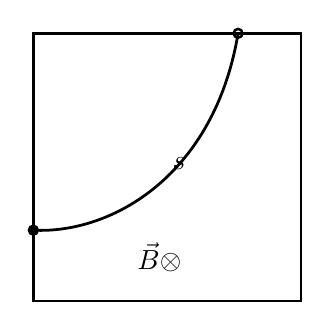
\begin{tikzpicture}[line width=0.9pt]
  % bounding square region
  \draw (0,0) rectangle (3.4,3.4);
  % field into page symbol and label
  \node at (1.6,0.55) {$\vec{B}\otimes$};
  % entry point on left edge (filled dot)
  \filldraw (0,0.9) circle (1.6pt);
  % curved trajectory (quarter-circle-like arc) from left edge to top edge
  \draw[line width=1pt] (0,0.9) .. controls (1.0,0.85) and (2.3,1.6) .. (2.6,3.4);
  \node at (1.85,1.75) {$s$};
  % exit point on top edge (open circle)
  \draw (2.6,3.4) circle (1.6pt);
\end{tikzpicture}
